\section{Testen von Hypothesen}

\begin{LA}
    {}{}
    Ein Losverkäufer hat mehrere tausend Lose. Er behauptet, dass 20\% seiner Lose Gewinnlose sind.

    \begin{enumerate}
        \item Du kaufst 100 Lose und erzielst nur 15 Gewinne.
              \begin{itemize}
                  \item Hältst du eine Beschwerde beim Losverkäufer für angebracht?
                  \item Wie gross ist die Wahrscheinlichkeit, dass du bei 100 Losen höchstens 15 Gewinne erzielst, wenn der Anteil der Gewinnlose tatsächlich 20\% beträgt?
              \end{itemize}

        \item Ändern sich die Berechnungen, wenn du beim Kauf von 200 Losen 30 Gewinne erzielst? Würdest du dich jetzt beschweren?

        \item Angenommen, du kaufst
              \begin{enumerate}
                  \item 100 Lose,
                  \item 200 Lose,
                  \item 500 Lose.
              \end{enumerate}
              Wie niedrig müsste jeweils die Anzahl von Gewinnlosen sein, damit du davon ausgehen kannst, dass der tatsächliche Anteil Gewinnlose bei weniger als 20\% liegt? \\
              Begründe deine Antworten auch rechnerisch.
    \end{enumerate}

\end{LA}

\clearpage

\subsection{Der Binomialtest}

Die sogenannte \textit{beurteilende Statistik} oder  \textit{schliessende Statistik} befasst sich mit der Frage, wie man Eigenschaften einer Stichprobe auf die Grundgesamtheit übertragen kann. Im Einführungsbeispiel besteht die Stichprobe aus den Losen die überprüft wurden. Die Grundgesamtheit sind alle Lose des Losverkäufers. Die Eigenschaft, die wir untersuchen ist der Anteil der Gewinnlose.

Diese Art der Fragestellung nennt man einen \textit{Hypothesentest}. Dabei wird eine Hypothese aufgestellt, die dann anhand der Stichprobe überprüft wird. In unserem Beispiel lautet die Hypothese, dass der Anteil der Gewinnlose kleiner als 20\% ist.

Solche Fragestellung kommen in vielen Bereichen zum Einsatz. Zum Beispiel:
\begin{itemize}
    \item Eine Umfrage ergibt, dass 55\% der Befragten für eine bestimmte Verfassungsänderung sind. Ist das Ergebnis repräsentativ für die gesamte Bevölkerung?
    \item Ein Medikament soll die Heilungschancen bei einer bestimmten Krankheit erhöhen. Bei einem Test mit 100 Patienten zeigt sich, dass 70\% der Patienten geheilt wurden. Von 100 nicht behandelten Patienten werden nur 60\% geheilt. Ist das Medikament wirksam?
    \item Verringert Vapen die Lebenserwartung?
    \item Sind Mädchen in der Schule besser als Jungen?
\end{itemize}


Im Folgenden soll das Vorgehen bei einem Hypothesentest an einem Beispiel illustiert werden:
\begin{bsp}
    {Binomialtest}{TestfürWürfel}
    Nachdem Alice einige Male in einem Würfelspiel gegen Bob verloren hat, vermutet sie, dass der verwendete Spielwürfel manipuliert ist. Sie denkt, dass die Wahrscheinlichkeit für eine Sechs nicht 1/6 beträgt. Um diese Hypothese zu überprüfen, beschliesst sie, den Würfel 100-mal zu werfen und dabei die Anzahl der Sechsen zu zählen. Vor dem Experiment bestimmt sie die folgenden Grössen:


    \begin{itemize}
        \item Nullhypothese \(H_0\):
        \item Alternativhypothese \(H_1\):
        \item Stichprobenumfang \(n\):
        \item 90\% Vorhersageintervall:
              \bigskip
        \item Verwerfungsbereich \(V\):
    \end{itemize}


    \vspace*{3cm}

    \begin{center}
        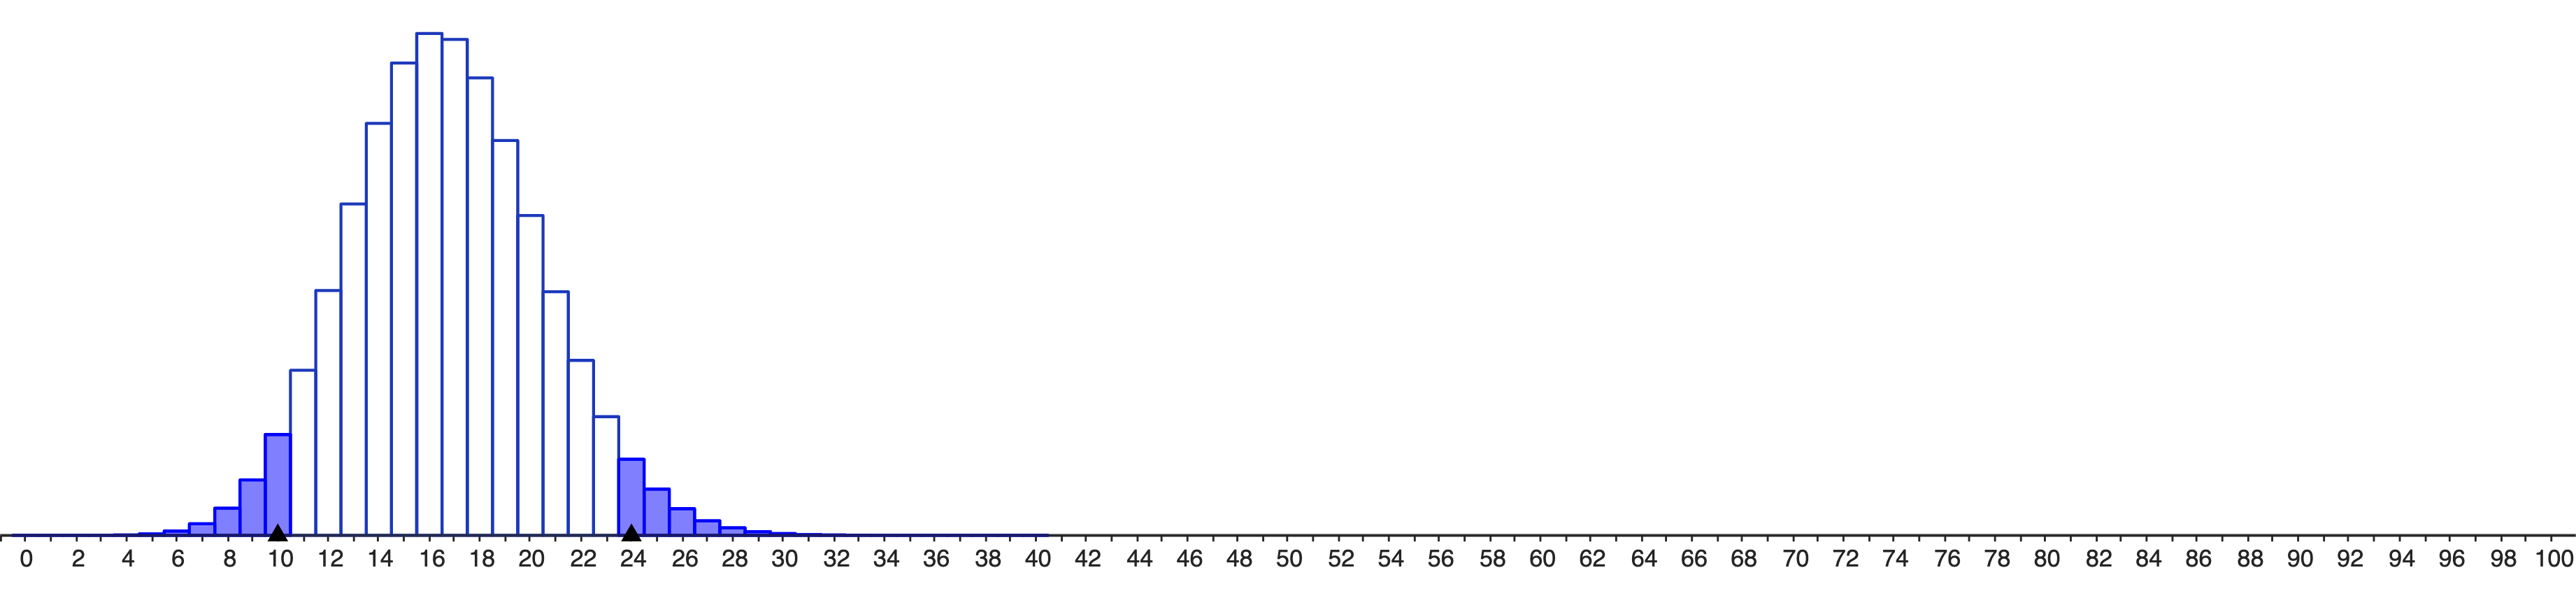
\includegraphics[width = 0.8\textwidth]{media/introBinomialtest.png}
    \end{center}

    Das Bild zeigt die Verteilung der Anzahl Sechsen unter Annahme, dass die Nullhypothese zutrifft. Die blaue Fläche ist der Verwerfungsbereich. Liegt das Ergebnis im Verwerfungsbereich, so wird die Nullhypothese verworfen. Liegt es ausserhalb, so wird die Nullhypothese beibehalten.
\end{bsp}



\begin{ueb}{}{}
    \begin{enumerate}
        \item Ein Glücksrad hat 16 gleich grosse Sektoren, von denen einer rot eingefärbt ist.
              Zeigt der Zeiger nach dem Drehen auf den roten Sektor, erzielt der Spieler einen Gewinn.
              Mit einem Test soll die Vermutung überprüft werden, dass die Wahrscheinlichkeit für einen Gewinn bei diesem Glücksrad nicht \( \frac{1}{16} \) ist.

              Konstruiere einen solchen Test: Gib die Nullhypothese an und bestimme ihren Verwerfungsbereich für den angegebenen Stichprobenumfang \( n \) auf Grundlage des 90\%-Vorhersageintervalls.
              \begin{enumerate}
                  \item \( n = 200 \)
                  \item \( n = 1000 \)
                  \item Welchen Schluss ziehst du, wenn das Ergebnis 25\% unter dem Erwartungswert liegt?
              \end{enumerate}

        \item Wasserverschmutzung durch chemische Substanzen kann langfristig dazu führen, dass sich die Geschlechterverteilung bei Fischen ändert.
              Anhand eines Probefangs von 50 Fischen soll überprüft werden, ob sich die Verteilung der Geschlechter bei einer Fischart in einem chemisch belasteten Fluss verändert hat.
              Normalerweise sind Männchen und Weibchen bei dieser Fischart gleich häufig.
              \begin{enumerate}
                  \item Entwirf einen entsprechenden Test auf Basis des 90\%-Vorhersageintervalls.
                  \item Entscheidet der Test, dass sich die Geschlechterverteilung verändert hat, so soll die Fabrik, die die Wasserverschmutzung verursacht hat, eine Geldstrafe zahlen. \\
                        Welche Argumente könnte die Fabrikleitung gegen die Geldstrafe vorbringen?
                  \item Wie könnte man den Test verändern, um die Gegenargumente der Fabrikleitung zu entkräften?
              \end{enumerate}
    \end{enumerate}

\end{ueb}

\clearpage
\emph{Lösungen:}
\begin{enumerate}
    \item
          \begin{enumerate}
              \item Nullhypothese \( H_0: p = \frac{1}{16} \). Alternativhypothese \(H_1: p\neq\frac{1}{16}\) \\
                    \( n = 200 \):\\
                    90\%-Intervall: ca.\ [7, 18] Treffer. \\
                    Verwerfungsbereich \(V=\{0, \dots 6\} \cup \{19, \dots 200\}\)

              \item Nullhypothese \( H_0: p = \frac{1}{16} \). Alternativhypothese \(H_1: p\neq\frac{1}{16}\) \\
                    \( n = 1000 \):\\
                    90\%-Intervall: ca.\ [50, 75] Treffer. \\
                    Verwerfungsbereich \(V=\{0, \dots 49\} \cup \{76, \dots 1000\}\)

              \item Bei 25\% weniger als dem Erwartungswert würde beim ersten Test die Nullhypothese beibehalten. Beim zweiten Test würde die Nullhypothese zugunsten der Alternativhypothese verworfen werden.
          \end{enumerate}

    \item
          \begin{enumerate}
              \item Nullhypothese \( H_0: p = 0.5 \). \\
                    90\%-Intervall für 50 Fische: ca.\ [19, 31] Männchen.
                    Verwerfungsbereich \(V=\{0, \dots 18\} \cup \{32, \dots 50\}\)

              \item \dots

              \item \dots
          \end{enumerate}
\end{enumerate}

\clearpage

























\subsection{Das Signifikanzniveau}

So wie wir den Binomialtest bisher verwendet haben, besteht eine grosse Gefahr, dass wir die Nullhypothese fälschlicherweise verwerfen. Beim \Cref{bsp:TestfürWürfel} mit dem Würfel würde ein tatsächlich fairer Würfel in 10\% der Fälle den Test nicht bestehen und zu unrecht als manipuliert gelten.

Je nach Anwendung kann dies schwerwiegende Folgen haben. Zum Beispiel könnte eine Fabrik, die keine Verantwortung für die Wasserverschmutzung trägt, zu Unrecht bestraft werden. Oder ein Medikament könnte als wirksam eingestuft werden, obwohl es tatsächlich keine Wirkung hat.

Aus diesem Grund werden Tests häufig so konstruiert, dass die Wahrscheinlichkeit, die Nullhypothese fälschlicherweise zu verwerfen, höchstens 5\% oder 1\% ist. Diese Wahrscheinlichkeit nennt man Signifikanzniveau.

\begin{definition}
    {Signifikanzniveau}{}
    Ein Hypothesentest hat ein Signifikanzniveau von \( \alpha \), wenn die Wahrscheinlichkeit, dass die Nullhypothese fälschlicherweise verworfen wird, höchstens \( \alpha \) ist.
\end{definition}

In der Praxis spricht man von einem \textit{signifikanten Resultat}, wenn bei einem Hypothesentest mit Signifikanzniveau \(\alpha \le 5\%\) die Nullhypothese verworfen wurde\footnote{Aus diesem Grund sagt man häufig auch, dass in etwa jeder 20. statistische Studie einen falschen Schluss gezogen wird\dots}. Ein Resultat ist \textit{sehr signifikant}, wenn das Signifikanzniveau \(\alpha \le 1\%\) ist, und  \textit{hoch signifikant}, bei \(\alpha \le 0.1\%\).

Will man einen Test mit einem Signifikanzniveau von \(\alpha=5\%\) durchführen, so muss man anstelle des 90\%-Vorhersageintervalls ein \(1-\alpha=95\%\)-Vorhersageintervall verwenden.

Tatsächlich kann jedem Intervall der Form \(\left\{\mu-k\cdot\sigma, \dots , \mu + k\cdot\sigma\right\}\) eine bestimmte Wahrscheinlichkeit zugeordnet werden, wobei diese Näherungen wieder umso besser sind, je grösser \(\sigma\) ist.

Die wichtigsten Werte sind in der folgenden Tabelle zusammengefasst:
\begin{satz}
    {\(\sigma\)-Umgebungen und Wahrscheinlichkeiten}{}
    Für eine binomialverteilte Zufallsvariable \(X\) mit \(\sigma > 3\) gilt:

    \begin{center}
        \begin{tabular}{{|c|c|}}
            \hline
            \(k\)    & \(P(\mu-k\cdot\sigma \le X \le \mu+k\cdot\sigma)\) \\ \hline
            \(1.28\) & \(\approx80\%\)                                    \\ \hline
            \(1.64\) & \(\approx90\%\)                                    \\ \hline
            \(1.96\) & \(\approx95\%\)                                    \\ \hline
            \(2.33\) & \(\approx98\%\)                                    \\ \hline
            \(2.58\) & \(\approx99\%\)                                    \\ \hline
        \end{tabular}
    \end{center}

    --> Ergänzen Sie die Tabelle in Ihrer Formelsammlung!
\end{satz}



\subsubsection*{Vorgehen bei einem Hypothesentest:}
\begin{enumerate}
    \item \emph{Wähle die Testparameter:}
          \begin{enumerate}
              \item \emph{Formuliere die Nullhypothese \(H_0\).} Diese ist das Gegenteil dessen, was vermutet oder gezeigt werden soll. Letzteres ist die Alternativhypothese \(H_1\).
              \item \emph{Wähle ein Signifikanzniveau \(\alpha\).} Je kleiner \(\alpha\), desto stichhaltiger ist ein Verwerfen der Nullhypothese. Gleichzeitig müssen die Resultate umso extremer sein, um die Nullhypothese verwerfen zu können.
              \item \emph{Wähle einen Stichprobenumfang.} Je grösser der Stichprobenumfang, desto genauer ist der Test.
          \end{enumerate}
    \item \emph{Bestimme den Verwerfungsbereich \(V\).} Berechne das \(1-\alpha\)-Vorhersageintervall und bestimme daraus den Verwerfungsbereich.
    \item \emph{Führe das Experiment durch und bestimme das Ergebnis.} Zähle die Anzahl der Erfolge in der Stichprobe. Je nachdem, ob das Ergebnis im Verwerfungsbereich liegt oder nicht, wird die Nullhypothese verworfen oder beibehalten.
\end{enumerate}
\begin{bsp}
    {Verdächtiger Würfel mit \(\alpha = 1\%\)}{}
    Bevor Alice Bob mit dem Verdacht konfrontiert, dass der Würfel manipuliert ist, möchte sie sicher sein, dass die Nullhypothese tatsächlich falsch ist. Sie entscheidet sich, den Würfel 200-mal zu werfen und dabei die Anzahl der Sechsen zu zählen. Sie verwendet ein Signifikanzniveau von \(\alpha = 1\%\). \\
    Beim Test zeigen 22 der Würfe eine Sechs.

    \begin{enumerate}
        \item Nullhypothese, Alternativhypothese, Signifikanzniveau und Stichprobenumfang:
              \[H_0: p = \frac{1}{6},\ H_1: p \neq \frac{1}{6},\ \alpha = 0.01,\ n = 200\]
        \item Verwerfungsbereich:
              \[\mu = np = 200 \cdot \frac{1}{6} = 33.\bar{3}, \qquad \sigma = \sqrt{npq} = \sqrt{200 \cdot \frac{1}{6} \cdot \frac{5}{6}} = 5.27\]
              Grenzen des 99\%-Vorhersageintervall (Tabelle \(\to\) Faktor \(2.58\)):
              \[\mu\pm2.58\sigma \approx 20 \text{ bzw. } 47\]
              Verwerfungsbereich:
              \[V = \{0, \dots, 19\} \cup \{48, \dots, 200\}\]
        \item Ergebnis:
              Da 22 nicht im Verwerfungsbereich liegt, wird die Nullhypothese beibehalten. Alice kann Bob also nicht beschuldigen, den Würfel manipuliert zu haben.
    \end{enumerate}

\end{bsp}
\clearpage
\begin{ueb}
    {}{}
    \begin{enumerate}
        \item Bei einem regelmässigen Körper sind die Seiten durchnummeriert. Er wird wie ein Würfel geworfen. Getestet wird die Nullhypothese «Eine Eins wird mit der Wahrscheinlichkeit \( p \) geworfen». \\
              Bestimme den Verwerfungsbereich für die angegebenen Werte.
              \begin{enumerate}
                  \item Werfen eines Tetraeders: \( n = 100, \ \alpha = 5\% \)
                  \item Werfen eines Oktaeders: \( n = 200, \ \alpha = 5\% \)
                  \item Werfen eines Dodekaeders (12-Flächner): \( n = 250, \ \alpha = 10\% \)
                  \item Werfen eines Ikosaeders (20-Flächner): \( n = 1000, \ \alpha = 1\% \)
              \end{enumerate}

        \item Hellseherei? Im Jahr 1973 führte Charles Tart ein Experiment an der University of California in Davis durch, um aussersinnliche Wahrnehmung zu demonstrieren. \\
              Er verwendete einen Zufallszahlengenerator auf einem Computer, der eines von vier möglichen Symbolen auswählte. \\
              Die Versuchsperson sah das Resultat nicht und musste das richtige Symbol herausfinden. \\
              Jede Versuchsperson wiederholte dies 500 Mal, und es wurden 15 Personen getestet, welche behaupteten, hellseherische Fähigkeiten zu besitzen. \\
              Insgesamt wurde das richtige Symbol in 2006 von \( 15 \cdot 500 = 7500 \) Wiederholungen herausgefunden (Freedman et al., 1978).

              \begin{enumerate}
                  \item Bestimme den Verwerfungsbereich der Nullhypothese «Die getesteten Personen erraten die Symbole rein zufällig» für das Signifikanzniveau \( \alpha = 1\% \).

                  \item Zu welchem Schluss führt der entwickelte Test?

                  \item Wie gross ist die Wahrscheinlichkeit, dass Personen ohne hellseherische Fähigkeiten bei 7500 Wiederholungen rein zufällig in 2006 oder mehr Fällen das richtige Symbol erraten?
              \end{enumerate}
    \end{enumerate}

\end{ueb}

\clearpage
\emph{Lösungen}
\begin{enumerate}
    \item
          \begin{enumerate}
              \item \(V=\{0, \dots, 16\} \cup \{34, \dots, 100\} \)
              \item \(V=\{0, \dots, 15\} \cup \{35, \dots, 200\} \)
              \item \(V=\{0, \dots, 13\} \cup \{29, \dots, 250\} \)
              \item \(V=\{0, \dots, 31\} \cup \{69, \dots, 1000\} \)
          \end{enumerate}
    \item \begin{enumerate}
              \item \(V=\{0, \dots, 1777\} \cup \{1973, \dots, 7500\} \)
              \item Die Nullhypothese wird verworfen!
              \item \(P(X\ge2006) \approx 0.03\%\).
          \end{enumerate}
\end{enumerate}





















\pagebreak
\subsection{Fehler 1. und 2. Art}
\begin{bsp}
    {Losverkäufer Teil 2}{}
    Ein Losverkäufer behauptet, 20\% der Lose seien Gewinnlose. Es werden 100 Lose getestet.
    \begin{itemize}
        \item Nullhypothese \( H_0 \): 20\% der Lose sind Gewinnlose.
        \item Gegenhypothese \( H_1 \): Der Anteil Gewinnlose ist nicht 20\%.
        \item Verwerfungsbereich: Wenn weniger als 10 Gewinnlose (oder mehr als 30) dabei sind, wird dem Losverkäufer misstraut.
    \end{itemize}


    Bei diesem Test kann es zufällig zu zwei möglichen Fehlschlüssen kommen:
    \begin{enumerate}
        \item Der Losverkäufer ist ehrlich, das Resultat des Tests liegt aber zufällig im Verwerfungsbereich. In anderen Worten: \(H_0\) wird fälschlicherweise verworfen.
        \item Der Losverkäufer ist unehrlich, das Resultat des Tests liegt aber zufälligerweise im Vorhersageintervall. In anderen Worten: \(H_0\) wird fälschlicherweise beibehalten.
    \end{enumerate}
\end{bsp}

\begin{definition}
    {Fehler 1. und 2. Art}{}
    \begin{itemize}
        \item  Ein Fehler 1. Art (oder auch \( \alpha \)-Fehler) liegt vor, wenn die Nullhypothese verworfen wird, obwohl sie in Wirklichkeit zutrifft.

              Die Wahrscheinlichkeit \( \alpha' \) für den Fehler 1. Art ist kleiner oder gleich dem Signifikanzniveau \( \alpha \).

        \item Ein Fehler 2. Art (oder auch \( \beta \)-Fehler) liegt vor, wenn die Nullhypothese beibehalten wird, obwohl sie in Wirklichkeit falsch ist.

              Die Wahrscheinlichkeit für den Fehler 2. Art wird mit \( \beta' \) bezeichnet.
              Für die Berechnung von \( \beta' \) muss eine Annahme über die tatsächliche Erfolgswahrscheinlichkeit getroffen werden.
    \end{itemize}


    \begin{center}


        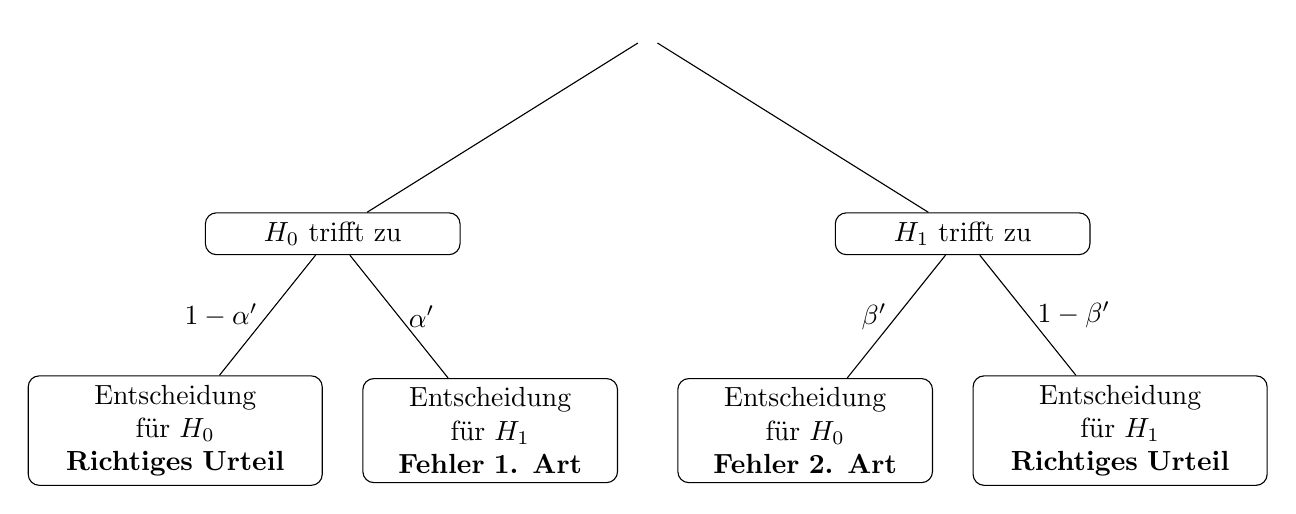
\begin{tikzpicture}[
                >=stealth, rounded corners,
                level 1/.style={sibling distance=8cm, level distance=2.5cm},
                level 2/.style={sibling distance=4cm, level distance=2.5cm}
            ]
            \node { }
            child {node[draw, rectangle, align=center, text width=3cm] {\(H_0\) trifft zu}
                    child {node[draw, rectangle, align=center, text width=3.5cm] {Entscheidung\\für \(H_0\)\\\textbf{Richtiges Urteil}}
                            edge from parent node[left] {\(1 - \alpha'\)}}
                    child {node[draw, rectangle, align=center, text width=3cm] {Entscheidung\\für \(H_1\)\\\textbf{Fehler 1. Art}}
                            edge from parent node[right] {\(\alpha'\)}}
                }
            child {node[draw, rectangle, align=center, text width=3cm] {\(H_1\) trifft zu}
                    child {node[draw, rectangle, align=center, text width=3cm] {Entscheidung\\für \(H_0\)\\\textbf{Fehler 2. Art}}
                            edge from parent node[left] {\(\beta'\)}}
                    child {node[draw, rectangle, align=center, text width=3.5cm] {Entscheidung\\für \(H_1\)\\\textbf{Richtiges Urteil}}
                            edge from parent node[right] {\(1 - \beta'\)}}
                };
        \end{tikzpicture}
    \end{center}


\end{definition}


\clearpage
\begin{bsp}
    {Berechnung von \(\alpha'\) und \(\beta'\)}{}
    Wir betrachten den folgenden Test:
    \begin{itemize}
        \item Eine Münze wird 100 mal geworfen. \( X \): Anzahl «Zahl».
        \item Nullhypothese \( H_0 \): Die Wahrscheinlichkeit für Zahl ist \( p = \frac{1}{2} \).
        \item Signifikanzniveau: \( \alpha = 5\% \).
        \item 95\%-Vorhersageintervall: \( I = \{40, 41, \ldots, 60\} \).
        \item Verwerfungsbereich: \( V = \{0, 1, \ldots, 39\} \cup \{61, 62, \ldots, 100\} \).
    \end{itemize}

    Die Wahrscheinlichkeit für den Fehler 1. Art ist die Wahrscheinlichkeit, dass das Ergebnis im Verwerfungsbereich zu liegen kommt, obwohl die Nullhypothese stimmt:
    \begin{align*}
        \alpha' & = P\left(X \in V \mid p=\frac{1}{2}\right)                                                  \\
                & = P\left(X \leq 39 \mid p=\frac{1}{2}\right) + P\left(X \geq 61 \mid p=\frac{1}{2}\right)   \\
                & = \mathrm{binomialCdf} (100, 0.5, 39) + \left(1 - \mathrm{binomialCdf}(100, 0.5, 60)\right) \\
                & \approx 3.52\%
    \end{align*}

    Für die Wahrscheinlichkeit \(\beta'\) für den Fehler 2. Art müssen wir eine Annahme treffen, wie gross \(p\) tatsächlich ist. In diesem Fall nehmen wir an, dass \(p=\frac{2}{3}\). Der \(\beta\)-Fehler entsteht dann, wenn die Nullhypothese falsch ist, dies jedoch vom Test nicht erkannt wird, weil das Ergebnis nicht im Verwerfungsbereich zu liegen kommt:
    \begin{align*}
        \beta' & = P\left(40 \leq X \leq 60 \,\big|\, p = \tfrac{2}{3}\right)             \\
               & = \mathrm{binomialCdf}(100, 2/3, 60)- \mathrm{binomialCdf}(100, 2/3, 39) \\
               & \approx 9.66\%
    \end{align*}
\end{bsp}


Idealerweise sind beide Fehlerwahrscheinlichkeiten klein. Veränderungen an einem Test haben die folgenden Auswirkungen auf die Fehlerwahrscheinlichkeiten \(\alpha'\) und \(\beta'\):
\begin{itemize}
    \item Verkleinerung des Verwerfungsbereichs:
          \begin{itemize}
              \item \( \alpha' \) wird kleiner
              \item \( \beta' \) wird grösser
          \end{itemize}

    \item Vergrösserung des Verwerfungsbereichs:
          \begin{itemize}
              \item \( \alpha' \) wird grösser
              \item \( \beta' \) wird kleiner
          \end{itemize}

    \item Einzige Option: Stichprobe \( n \) vergrössern.
\end{itemize}

\clearpage
\begin{ueb}
    {}{}
    \begin{enumerate}
        \item Ein Würfel soll in 50 Würfen auf einem Signifikanzniveau von 5\% darauf geprüft werden, ob die Wahrscheinlichkeit für eine Sechs tatsächlich \( p = \frac{1}{6} \) beträgt. Als Verwerfungsbereich wird
              \[
                  V_{H_0} = \{0, \ldots, 3\} \cup \{15, \ldots, 50\}
              \]
              gewählt.
              \begin{enumerate}
                  \item Bestimme die Wahrscheinlichkeit für einen Fehler 1. Art.
                  \item Tatsächlich beträgt die Wahrscheinlichkeit für eine Sechs \( p = 0.25 \). Mit welcher Wahrscheinlichkeit wird der Testwürfel trotzdem als fair eingestuft?
              \end{enumerate}

        \item Eine Münze soll in 100 Würfen auf einem Signifikanzniveau von 10\% darauf getestet werden, ob die Wahrscheinlichkeiten für Kopf und Zahl gleich gross sind.
              \begin{enumerate}
                  \item Gib die Nullhypothese und die Gegenhypothese an und bestimme den Verwerfungsbereich.
                  \item Bestimme die Wahrscheinlichkeit für einen Fehler 1. Art.
                  \item Die Münze zeigt mit einer Wahrscheinlichkeit von \( p = 0.4 \) Zahl. Wie gross ist die Wahrscheinlichkeit, dass der Test zu einer Fehlentscheidung führt?
                  \item Wie verändern sich  \( \alpha' \) und \( \beta' \), wenn \(n=200\) bzw \(n=300\)?
                  \item Wie hoch muss \(n\) mindestens sein, damit \( \beta'<1\%\) ist?
                        \\ Tipp: Sie können \(n\) durch Ausprobieren bestimmen oder mit dem Computer:
                        \begin{itemize}
                            \item In Excel kann die kumulative Binomialverteilung mit der Funktion \texttt{BINOM.VERT(x; n; p; WAHR)} berechnet werden.
                            \item In \href{https://webtigerpython.ethz.ch}{Python} kann die kumulative Binomialverteilung mit
                                  \begin{lstlisting}[language = Python]
from scipy.stats import binom  # import der Funktion binom
binom.cdf(x, n, p)  # berechnet P(X <= x) 
\end{lstlisting}
                                  berechnet werden.
                        \end{itemize}

              \end{enumerate}
    \end{enumerate}

\end{ueb}

\emph{Lösungen:}
\begin{enumerate}
    \item \begin{enumerate}
              \item 3.8\%
              \item 74.8\%
          \end{enumerate}
    \item \begin{enumerate}
              \item \(H_0: p=0.5\), \(H_1: p\neq0.5\), \( V = \{0, 1, \ldots, 41\} \cup \{59, 62, \ldots, 100\} \)
              \item 8.86\%
              \item 37.7\%
              \item \begin{itemize}
                        \item \(n=200: \alpha' =7.68\% , \beta'=13.97\%\)
                        \item \(n=300: \alpha' = 9.39\%, \beta'=3.45\%\)
                    \end{itemize}
              \item \(n = 392 \Rightarrow \beta'\approx 0.009971751\)
          \end{enumerate}
\end{enumerate}
























\clearpage
\subsection{Einseitige Tests}
Bisher hat Alice die Hypothese geprüft, dass Bobs Spielwürfel so manipuliert ist, dass die Wahrscheinlichkeit für eine Sechs nicht \(p=1/6\) ist.

Dabei hat sie die Nullhypothese verworfen, wenn in der Stichprobe zu viele oder zu wenige Sechsen geworfen wurden. Das Bild zeigt in blau den Verwerfungsbereich für diesen Test:
\begin{center}
    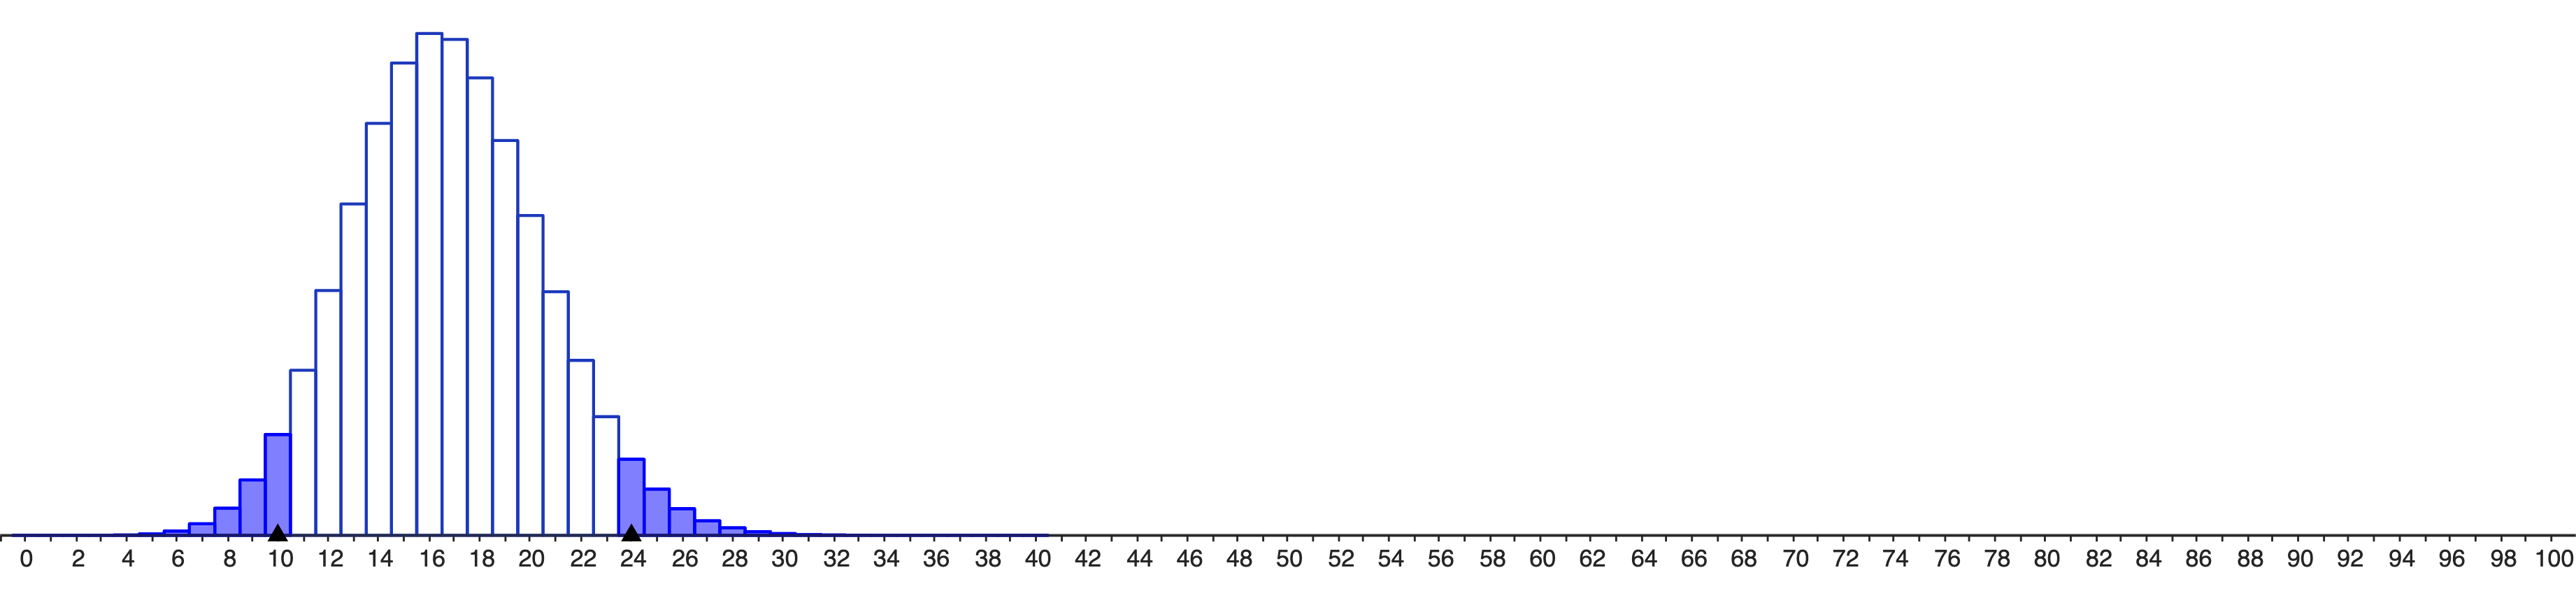
\includegraphics[width = 0.8 \textwidth]{media/introBinomialtest.png}
\end{center}

Ihr eigentlicher Verdacht ist jedoch, dass die Sechs zu selten erscheint! Ihre Vermutung ist daher \(H_1: p < 1/6\). Die Nullhypothese lautet in diesem Fall \(H_0: p \ge 1/6\). Die Nullhypothese soll nur verworfen werden, wenn die Anzahl Sechsen zu tief ist:

\begin{center}
    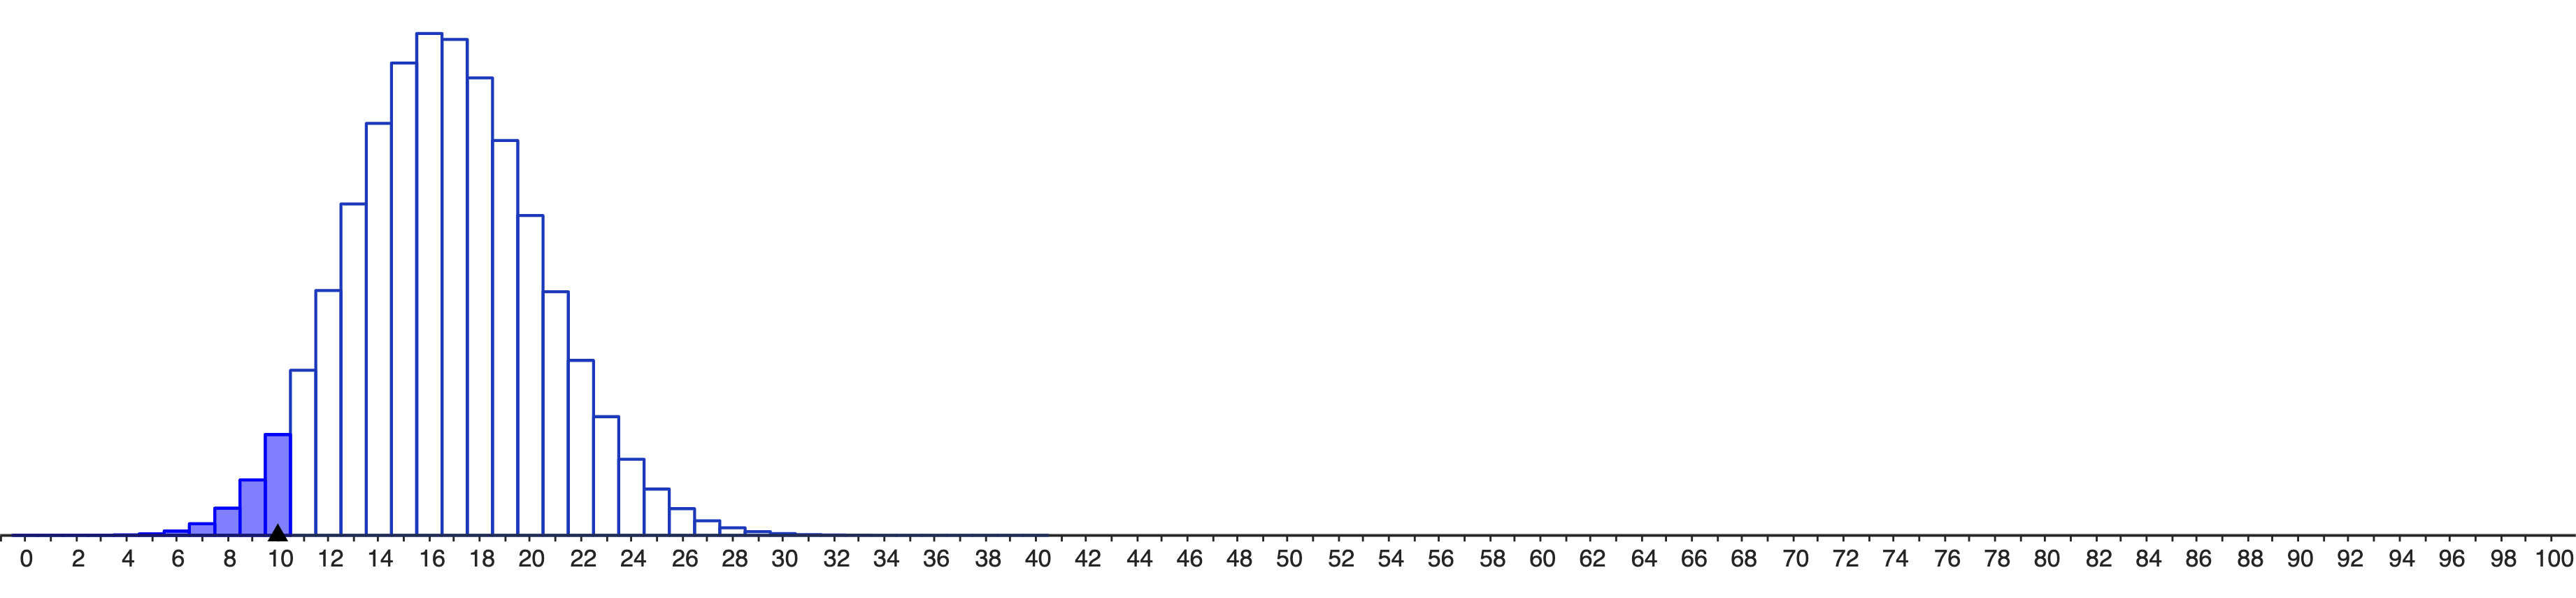
\includegraphics[width = 0.8 \textwidth]{media/linkssitigerTest.png}
\end{center}

Beachte: Weil die Verteilung nahezu symmetrisch ist, ist für das Signifikanzniveau \(\alpha\) die Grenze des \(1-2\alpha\) Vorhersageintervall entscheidend.

\begin{center}


    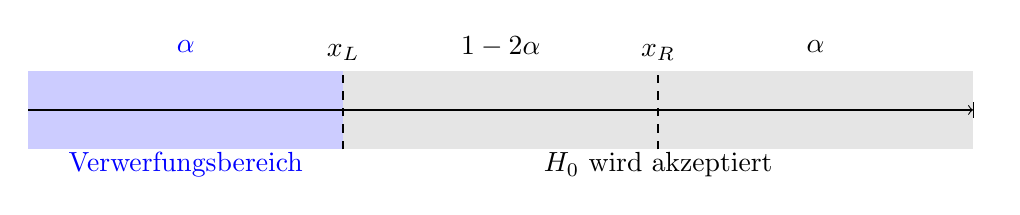
\begin{tikzpicture}

        % Achse


        % Markierungen und Beschriftungen
        \foreach \x in {0,...,12}
        \draw (\x,0.1) -- (\x,-0.1);

        % Rote Zone links
        % \fill[red!20] (0,-0.5) rectangle (4,0.5);
        % \node[red!60!black] at (2,-0.7) {Verwerfungsbereich};
        % \node[red!60!black] at (2,0.8) {$\alpha'$};
        \fill[blue!20] (0,-0.5) rectangle (4,0.5);
        \node[blue] at (2,-0.7) {Verwerfungsbereich};
        \node[blue] at (2,0.8) {\(\alpha\)};

        % Graue Zone Mitte
        \fill[gray!20] (4,-0.5) rectangle (8,0.5);
        \node at (6,0.8) {\(1-2\alpha\)};
        \node at (8,-0.7) {\(H_0\) wird akzeptiert};

        % Graue Zone rechts
        \fill[gray!20] (8,-0.5) rectangle (12,0.5);
        \node at (10,0.8) {\(\alpha\)};
        \node at (10,-0.7) {};

        % Schwellen
        \draw[thick, dashed] (4,-0.5) -- (4,0.5) node[above] {\(x_L\)};
        \draw[thick, dashed] (8,-0.5) -- (8,0.5) node[above] {\(x_R\)};

        % Achsenbeschriftungen unten
        % \node at (0,-0.3) {0};
        % \node at (2,-0.3) {5};
        % \node at (4,-0.3) {10};
        % \node at (6,-0.3) {15};
        % \node at (8,-0.3) {20};
        % \node at (10,-0.3) {25};
        % \node at (12,-0.3) {30};

        \draw[->] (0,0) -- (12,0) node[anchor=west] {};

    \end{tikzpicture}
\end{center}

\clearpage
\begin{bsp}
    {Einseitiger Test für den verdächtigen Würfel}{}
    Testparameter bestimmen:
    \begin{itemize}
        \item \( H_0 : p \ge \frac{1}{6},\; n = 100,\; \alpha = 10\% \)
        \item Linke Grenze des 80\%-Vorhersageintervalls (Tabelle --> Faktor 1.28):
              \[
                  x_L = \frac{100}{6} - 1.28 \cdot \sqrt{100 \cdot \frac{1}{6} \cdot \frac{5}{6}} \approx 11.9 \approx 12
              \]
        \item Verwerfungsbereich:
              \[
                  V = \{0, 1, 2, \ldots, 11\}
              \]
    \end{itemize}

    Berechnung der Fehlerwahrscheinlichkeiten:
    \begin{itemize}
        \item Fehler erster Art \\
              Annahme \( p = \frac{1}{6} \) \\
              \(\alpha' = P(X \in V) = P(X \le 11) \approx 0.0777 \)

        \item Fehler zweiter Art bei \( p = \frac{1}{10} \) \\
              \(\beta' = P(X \notin V) = P(X \ge 12) = 1 - P(X \le 11) \approx 0.297 \)
    \end{itemize}
\end{bsp}
\clearpage
\begin{ueb}
    {}{}
    \begin{enumerate}
        \item Ein Casino behauptet, dass bei seinen Glücksspielautomaten die Wahrscheinlichkeit für einen Gewinn bei (mindestens) 25\% liege. Diese Angabe soll mit einer Serie von \( n \) Spielen getestet werden. Gehe wie folgt vor:
              \begin{itemize}
                  \item Konstruiere einen statistischen Test zur angegebenen Gegenhypothese und zum Stichprobenumfang \( n \) (\( \alpha = 5\% \)).
                  \item Bestimme für die konstruierten Tests den Fehler zweiter Art für den Fall, dass die Gewinnwahrscheinlichkeit tatsächlich \( p_1 = 15\% \) (bzw. \( p_2 = 20\% \)) beträgt.
              \end{itemize}
              \begin{enumerate}
                  \item \( H_1 : p \neq 25\% \) (zweiseitig), \( n = 100 \)
                  \item \( H_1 : p < 25\% \) (einseitig), \( n = 100 \)
              \end{enumerate}
        \item Gemäss Angaben des Herstellers treten bei höchstens 10\% der Patienten, die ein bestimmtes Medikament erhalten, Nebenwirkungen auf. Eine Chefärztin des Spitals vermutet, dass bei ihren Patienten dieser Anteil höher ist. Um diese Vermutung zu überprüfen, werden 120 Patienten untersucht, denen das Medikament verabreicht worden ist.
              \begin{enumerate}
                  \item Stelle Nullhypothese und Gegenhypothese für einen entsprechenden Test auf.
                  \item Beschreibe, welche Folgen der Fehler 1. Art und der Fehler 2. Art bei diesem Test haben.
                  \item Berechne die Verwerfungsbereiche für die folgenden Signifikanzniveaus: \(\alpha = 10\%\), \(\alpha = 5\%\) und \(\alpha = 1\%\). Bestimme jeweils die Wahrscheinlichkeit \(\beta\) eines Fehler 2. Art unter der Annahme, dass der Anteil von Patienten mit Nebenwirkungen tatsächlich 20\% beträgt.
                  \item Die Ärztin stellt bei 19 Patienten Nebenwirkungen fest. Welche Schlüsse kann sie daraus ziehen? Unterscheide die drei Fälle \(\alpha = 10\%\), \(\alpha = 5\%\) und \(\alpha = 1\%\).
                  \item Worauf muss bei der Festlegung von \(\alpha\) bei diesem Medizintest geachtet werden? Welches \(\alpha\) ist hier sinnvoll und wieso?
              \end{enumerate}
    \end{enumerate}

\end{ueb}

\clearpage
\emph{Lösungen:}
\begin{enumerate}
    \item

          \begin{enumerate}
              \item \(V=\{0,\dots, 16\} \cup \{34,\dots, 100\}, \qquad \beta_1\approx 32.75\%, \beta_2 \approx 80.69\%\)
              \item  \(V=\{0,\dots, 17\} , \qquad \beta_1\approx 23.67\%, \beta_2 \approx 72.88\%\)
          \end{enumerate}
    \item \begin{enumerate}
              \item \(H_0: p\le 10\%, \qquad h_1: p > 10\%\)
              \item Fehler 1. Art: Das Medikament wird nicht mehr verabreicht, obwohl es selten Nebenwirkungen hat.\\
                    Fehler 2. Art: Das Medikament wird weiter verabreicht, obwohl es häufig Nebenwirkungen verursacht.
              \item \begin{itemize}
                        \item \(\alpha = 0.1 \Rightarrow V = \{17, \dots, 120\} \quad \beta \approx 3.88\%\)
                        \item \(\alpha = 0.05 \Rightarrow V = \{18, \dots, 120\} \quad \beta \approx 6.47\%\)
                        \item \(\alpha = 0.01 \Rightarrow V = \{21, \dots, 120\} \quad \beta \approx 21.46\%\)
                    \end{itemize}
              \item
                    \begin{itemize}
                        \item \(\alpha = 0.1\) Das Resultat spricht dafür, dass bei mehr als 10\% der Patienten Nebenwirkungen auftreten.
                        \item \(\alpha = 0.05\) Das Resultat spricht dafür, dass bei mehr als 10\% der Patienten Nebenwirkungen auftreten.
                        \item \(\alpha = 0.01\) Das Resultat spricht dafür, dass bei höchstens 10\% der Patienten Nebenwirkungen auftreten.
                    \end{itemize}
              \item In diesem Fall ist (vermutlich) wichtiger, dass \(\beta\) klein ist, weil sonst die Gefahr von Nebenwirkungen droht. Das Signifikanzniveau \(\alpha\) darf darum nicht zu klein sein.
          \end{enumerate}
\end{enumerate}